
\section{Introduction}
\paragraph{}
Ce projet a été réalisé par quatre étudiants de première année de
Master Informatique de l'Université de Bordeaux (spécialité Génie
Logiciel), dans le cadre de l'UE Projet de Programmation.

\subsection{Un outil pour assister l'improvisation musicale}
\paragraph{}
Le projet a été proposé par Myriam Desainte-Catherine, chercheur au
Studio de Création et de Recherche en Informatique et Musiques
Expérimentales (SCRIME) et enseignante à l'ENSEIRB-MATMECA, et Yacine
Amarouchene, physicien du Laboratoire d'Onde et Matière d'Aquitaine
(LOMA). Il a été pensé comme un outil d'aide à "l'improvisation
musicale", un dispositif permettant d'aider un groupe de musiciens à
improviser mais permettant aussi de mieux comprendre la nature de
l'improvisation en musique.

\subsection{Improvisation et corrélation}
\paragraph{}
Il est essentiel de comprendre ces deux notions afin de bien situer
l'intérêt du projet ; elles sont le c\oe ur de notre travail.
\paragraph{}
Lors d'une improvisation en groupe, des musiciens jouent sans règle
établie ; ils cherchent alors à fournir à leur auditoire une
production cohérente, ou du moins au sein de laquelle chaque musicien
joue un rôle dans l'harmonie du morceau en s'accordant avec ses
pairs. La relation qui unit le jeu de deux musiciens et évalue la
qualité de leur accord porte un nom : c'est la corrélation.
\paragraph{}
Au sens premier et basique du terme, la corrélation est le rapport
réciproque entre deux éléments. En statistiques, on parle souvent de
corrélation pour mesurer l'intensité de la liaison existant entre deux
variables. Dans le cadre de l'étude de signaux sonores, les
traductions graphiques de ces signaux par transformée de Fourier
peuvent jouer le rôle des courbes dont on mesure la corrélation.
\paragraph{}
En musique, il n'existe pas une mais un nombre indéfini de "fonctions
de corrélation" potentiellement existantes, dont la complexité et les
paramètres varient. "Comprendre" la corrélation et l'improvisation,
dans le cadre de ce projet, c'est aussi trouver, inventer la fonction
de corrélation qui répond le mieux aux besoins d'un groupe
d'improvisateurs. Une bonne fonction de corrélation, dans ce cadre
spécifique, est une fonction qui fait en sorte qu'un groupe de
musiciens joue un morceau plus satisfaisant lorsque ses membres sont
davantage corrélés.

\subsection{L'existant}
\paragraph{}
Ce projet a été initié par les clients précédemment cités il y a plus
d'un an. Nous sommes le troisième groupe à travailler sur ce projet et
développons donc sur la base des travaux réalisés successivement par
nos prédécesseurs.

\subsubsection{Premiers travaux réalisés sur le projet}
\paragraph{}
Les premiers travaux portant sur ce projet ont été réalisés par un
groupe de six étudiants de l'ENSEIRB-MATMECA. Cette équipe est la
première à réaliser un programme informatique analysant et comparant
des pistes mono-instrumentales pour évaluer leurs corrélations. Ce
programme, prenant en entrées des pistes sonores, retourne une matrice
graphique prenant les mêmes pistes en abscisses et en ordonnées et
retournant pour chaque case une couleur permettant d'évaluer la
corrélation existant entre les deux pistes correspondantes grâce à un
code précis.

  \begin{figure}[h]
    \centering
    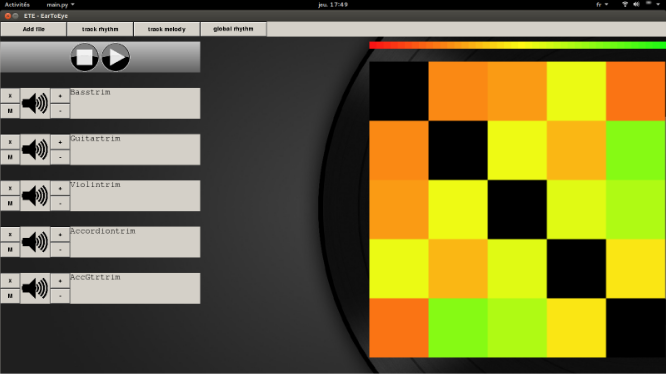
\includegraphics[scale=0.5]{matriceenseirb.png}
    \caption{Capture d'écran du projet mené par les étudiants de l'ENSEIRB}
    \label{matrice-enseirb}
  \end{figure}

\paragraph{}
Ci-dessus, la matrice obtenue à l'issue d'un test du programme. Plus
la couleur d'une case est proche du vert, plus la corrélation entre
les deux pistes correspondant au point d'abscisse et au point
d'ordonnée est élevée. À l'inverse, une case dont la couleur est
proche du rouge indique que les deux pistes évaluées sont
décorrélées. La corrélation d'une piste mono-instrumentale avec
elle-même, qui donne toujours un résultat maximal, n'est pas calculée,
ce qui se traduit sur le résultat graphique ci-dessus par une
diagonale de cases noires. La matrice de corrélation est donc
systématiquement symétrique.

\subsubsection{Le système embarqué BELA}
\paragraph{}
Avant de confier la suite du projet à d'autres étudiants, nos clients
ont choisi de le rendre plus fonctionnel grâce à l'emploi d'un système
embarqué particulier : BELA.

\begin{figure}[h]
    \centering
    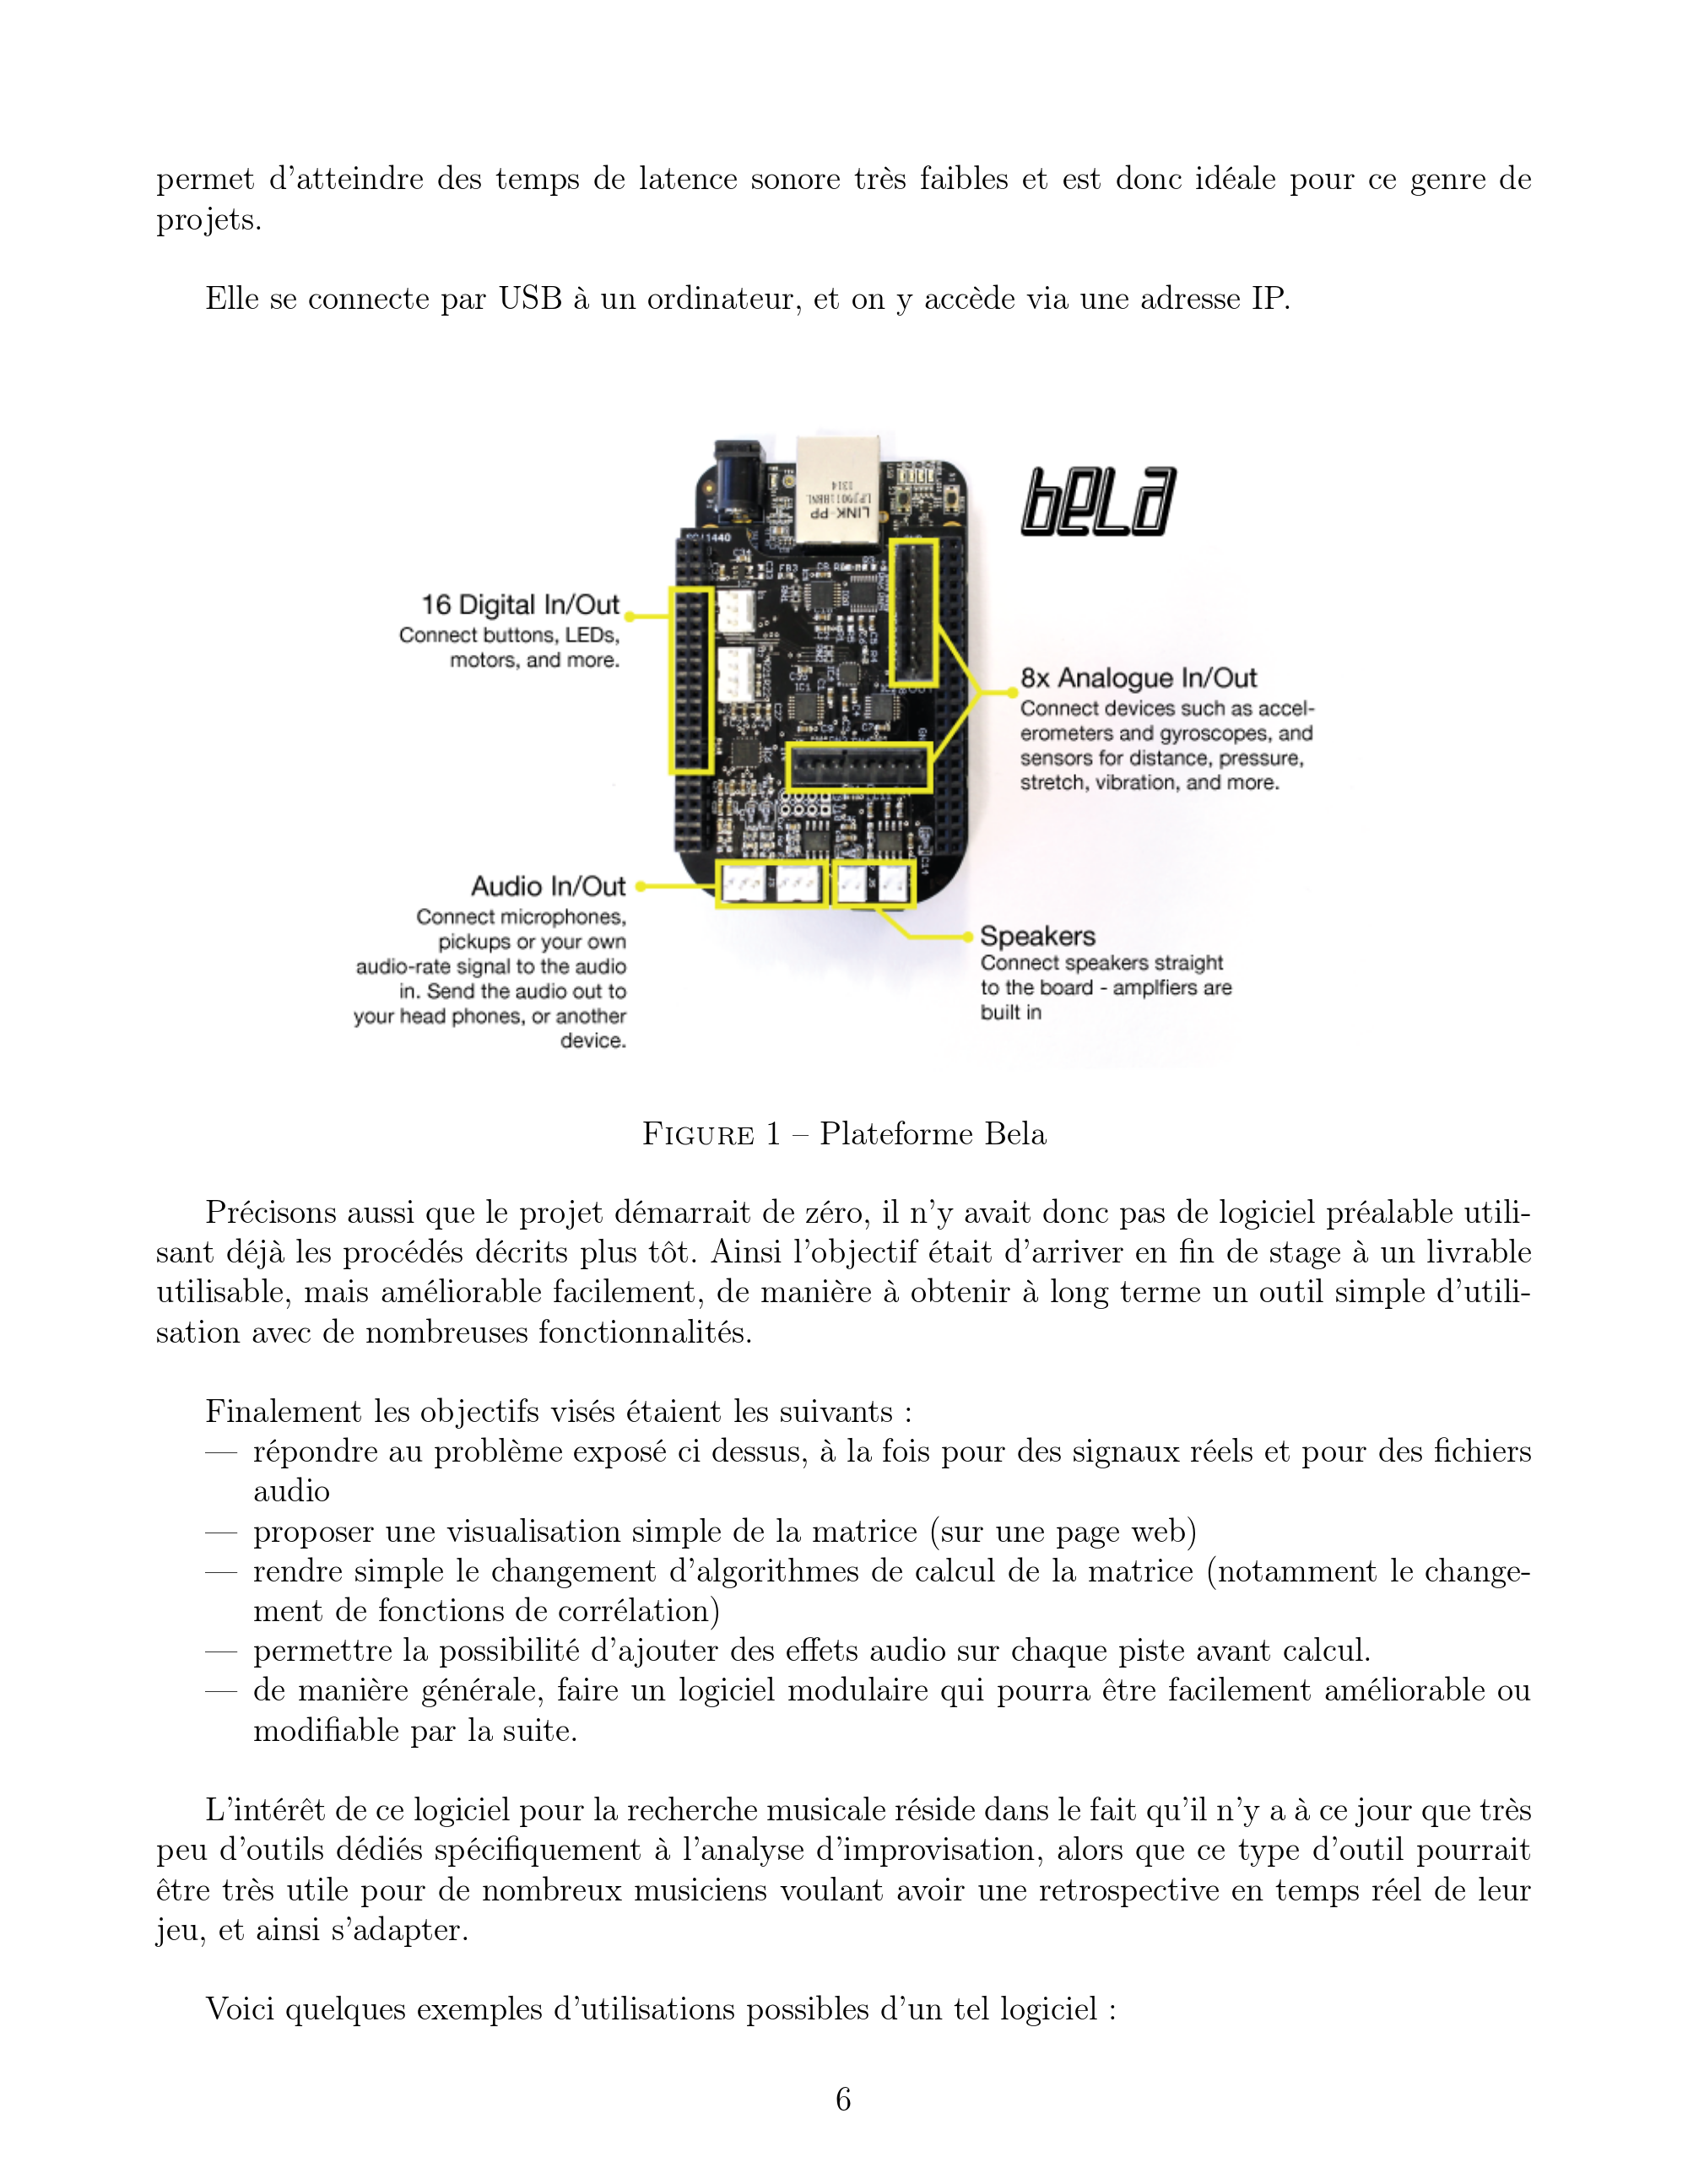
\includegraphics[scale=0.5]{bela.png}
    \caption{Capture de la documentation proposée par le site officiel de Bela}
    \label{bela}
  \end{figure}

\paragraph{}
L'aperçu du dispositif externe de BELA présenté ci-dessus témoigne
notamment de la présence d'entrées analogiques pour connecter des
instruments électriques ou enregistreurs sonores. On comprend alors
que le rôle de BELA au sein de ce projet est l'utilisation d'un
programme similaire à celui implémenté par les étudiants de l'ENSEIRB
en temps réel par un groupe d'improvisateurs, dont les instruments
seraient connectés à cet outil. Ce dernier dispose déjà de fonctions
de traitement du son codées en C++, mais revêt surtout un intérêt pour
les développeurs, qui peuvent librement modifier et enrichir son
programme.

\subsubsection{Un logiciel d'aide à l'improvisation musicale}
\paragraph{}
En juin 2017, Jérémy Lixandre, membre des six étudiants ayant amorcé
le projet, poursuit seul ces travaux en s'aidant cette fois de BELA,
au cours d'un stage de deux mois au laboratoire du SCRIME de
Bordeaux. Il reprend le concept de "matrice de corrélation" mais
doit reprendre l'implémentation du logiciel à zéro, puisqu'il
abandonne le langage Python utilisé lors des premiers travaux pour
passer à la programmation C++ exigée par le code de BELA.
\paragraph{}
De plus, il relègue les travaux de recherche sur la corrélation et ses
formules, des tâches relevant de la physique et des mathématiques, au
second plan pour mener un projet essentiellement logiciel. En
utilisant le code de BELA, il recrée un outil permettant d'analyser la
corrélation de signaux sonores et d'afficher la matrice de corrélation
présentée plus haut. Seulement cette fois, les signaux sonores traités
proviennent de BELA et peuvent donc être produits par des instruments
branchés directement sur le système. Ce nouveau programme permet donc
à des musiciens d'avoir un retour visuel en temps réel de leur
improvisation, et peut même comparer des pistes mono-instrumentales
jouées en temps réel avec des fichiers sonores numériques déjà
existant.

\subsubsection{Détails sur le programme existant}
\paragraph{}
Le programme développé par Jérémy s'intitule \verb!VisualImpro!. Il se
veut "générique", a été implémenté de sorte à permettre à des
développeurs de l'améliorer et de le modifier facilement, et à des
utilisateurs renseignés de modifier certains paramètres et
configurations liés aux calculs de la matrice. Son architecture
logicielle constitue le socle de notre travail, c'est elle que nous
allons devoir ré-organiser et enrichir, afin notamment d'ajouter de
nouvelles fonctionnalités au programme.
\paragraph{}
Le code du programme doit notamment contenir trois fichiers .cpp dont
les noms sont \verb!Prepoc*.cpp!, \verb!Coeff*.cpp! et
\verb!Color*.cpp! et qui contiennent respectivement la fonction de
"pre-processing" ou traitement du signal en amont, la fonction de
calcul du coefficient de corrélation et la fonction associant un
coefficiant à une couleur. Le programme est construit de sorte à ce
que tout fichier respectant ce nommage puisse être ajouté au programme
afin de permettre à un utilisateur de choisir la fonction de
\textit{pre-processing}/calcul de coefficiant de
corrélation/traduction en couleur de son choix.
\begin{itemize}
 \item La fonction \verb!Preproc! prend en entrée une matrice de
       vecteurs représentant les signaux d'entrée. Elle retourne une
       nouvelle matrice de vecteurs, qui pourra présenter des
       échantillons de plus petite taille que la matrice d'entrée par
       exemple, dans un souci d'optimisation des performances du
       programme.
 \item La fonction \verb!Coeff! prend en entrée deux vecteurs
       (appartenant à la matrice de sortie précédemment abordée) et
       retourne une valeur comprise entre 0 et 1 et correspondant à la
       corrélation établie entre les deux signaux traités. On peut
       imaginer une infinité potentielle de calculs pour donner lieu à
       une corrélation dans le cadre de ce programme ; il s'agit de
       calculs relativement arbitraires qui seront décrits plus en détail
       dans la suite de ce mémoire.
 \item La fonction \verb!Color! prend le coefficient précédemment obtenu
       pour entrée et retourne un triplet RGB ; il s'agit d'un objet C++
       défini par l'une des classes du programme.
\end{itemize}
Ces trois fichiers sont répertoriés dans un dossier \verb!process!. Un
fichier de configuration permet d'écrire quel fichier choisir pour
chacune des trois fonctions.

\paragraph{}
Le seul fichier imposé par l'IDE de Bela se nomme \verb!render.cpp!. Il
contient lui-même trois fonctions :
\begin{itemize}
 \item La fonction \verb!setup()! initialise et prépare les ressources de
       traitement du son.
 \item La fonction \verb!render()! s'appelle de manière régulière et répétée
       tout au long du processus audio. Elle a pour arguments des buffers
       contenant les échantillons à traiter.
 \item La fonction \verb!cleanup()! est appelée à la fin du processus pour
       libérer les ressources allouées et mettre fin à certaines tâches.
\end{itemize}

\paragraph{}
Une structure \verb!AuxiliaryTask! est mise à la disposition du
programmeur et est destinée à répertorier des fonctions trop coûteuses
en temps à l'exécution pour le code de \verb!render.cpp!.

\paragraph{}
Le fichier \verb!main.cpp!, en plus de lancer le programme, fait office de
fichier de configuration. L'utilisateur peut y entrer les noms des
fonctions de \textit{pre-processing}/calcul de coefficient/calcul de
triplet RGB de son choix. D'autres configurations purement relatives
au traitement de l'audio peuvent être modifiées dans le fichier
render.cpp.

\subsubsection{Motivation, intérêt et avenir du programme VisualImpro}
\paragraph{}
Le programme a été développé dans le but de fournir une rétrospective
visuelle en temps réel à des musiciens jouant en même temps et censée
évaluer leur improvisation. La fonction de corrélation, le critère de
cette évaluation, doit être modifiable selon les objectifs de
l'utilisateur, car aucune science exacte ne saurait vraiment évaluer
la qualité de l'harmonie existant entre les jeux de deux
musiciens. Plutôt que de leur indiquer la qualité de leur
improvisation comme elle pourrait le laisser penser, la matrice
graphique doit informer les musiciens sur la nature même de
l'improvisation. En observant la matrice tout en jouant pour une
configuration du logiciel donné, les musiciens pourraient non
seulement établir des liens entre l'évaluation de la corrélation entre
leurs jeux respectifs et le son qu'ils produisent, mais également
comprendre le fonctionnement du logiciel lui-même, et en s'adaptant
progressivement pour améliorer ces indices de corrélation, déterminer
si la configuration choisie leur convient et produit un résultat
agréable à l'oreille dans leur façon de jouer.

\begin{figure}[h]
    \centering
    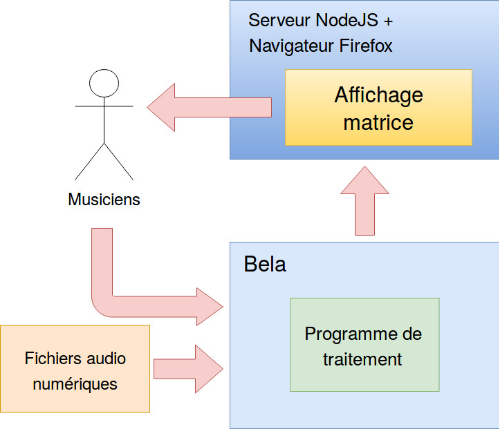
\includegraphics[scale=0.5]{schemaglobal.png}
    \caption{Schéma global du dispositif de \verb!VisualImpro!}
    \label{schéma global}
  \end{figure}
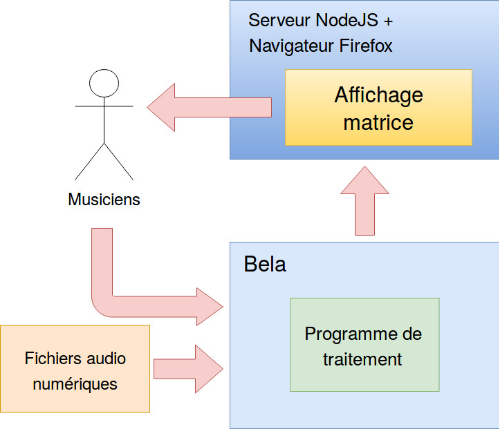
\includegraphics[scale=1]{schemaglobal.png}

\paragraph{}
Ci-dessus, un schéma global du fonctionnement du dispositif. Les
musiciens jouent un morceau traité par Bela qui, via l'intermédiaire
d'une machine, affiche sur le navigateur web Mozilla Firefox la
matrice graphique de corrélations censée assister le jeu des
musiciens.

\paragraph{}
Différentes pistes ont été proposées par Jérémy dans son rapport pour
améliorer le logiciel produit : implémenter un retour sonore indiquant
aux musiciens la qualité des corrélations en fonction du coefficient
calculé à la place du retour visuel, ajouter des effets audio aux
pistes sonores en amont du calcul de corrélation...

\subsection{La rédaction du cahier des besoins}

\paragraph{}
Durant les premières semaines de travail sur ce projet, il nous a
fallu établir précisément ses besoins, tâche qui a suscité débats et
questionnements et s'est révélée plus difficile que prévu. Appréhender
l'intérêt du projet ou le fonctionnement de l'existant exigeaient
déjà, en soit, une certaine réflexion.

\subsubsection{Les premiers besoins fonctionnels listés par nos clients}
\paragraph{}
Après les premières entrevues avec les deux professeurs à l'origine du
projet, l'objectif principal qui se dessine est l'implémentation d'un
retour sonore sur la sortie audio dont dispose le système
embarqué. Grâce à la technologie de Bela, on devrait être en mesure de
remplacer ou compléter le retour visuel par une évaluation audio du
jeu des musiciens.
\paragraph{}
Ce qui motive ce besoin particulier est l'intérêt technologique que
représente l'utilisation de Bela pour produire un résultat sonore
dépendant de nos traitements de calcul mais également de fournir une
assistance aux musiciens supposée plus efficace qu'un simple affichage
visuel. En effet, lorsqu'un groupe tente d'improviser ensemble, il ne
doit pas être évident pour ses membres de se focaliser sur un code
couleur ou un affichage visuel dynamique pour adapter et réviser leurs
jeux. Ce sur quoi se basent usuellement des musiciens tentant de
s'accorder les uns avec les autres sans partition ou chef d'orchestre,
c'est bien évidemment le son, celui que produisent les autres. Avec
l'implémentation de cette sortie sonore, qui serait une version
modifiée en temps réel du morceau joué en entrée du système, on tente
de dénaturer cette logique et d'apporter aux musiciens une nouvelle
façon d'improviser qui, selon les configurations du logiciel choisies,
pourra se révéler plus efficace. Ce nouvel outil mérite quelques
éclaircissements quant à son fonctionnement et son intérêt global.
\paragraph{}
Dans sa version du logiciel, Jérémy avait anticipé et prévu dans son
implémentation la possibilité de produire un retour sonore dépendant
directement du coefficient de corrélation. Son idée était d'émettre un
signal dont l'amplitude varierait de manière proportionnelle et en
temps réel à un coefficient (ou à une somme des coefficients) de
corrélation. Ainsi, par-dessus le morceau qu'ils seraient en train de
jouer, les musiciens entendraient ce "signal", ce bruit évaluant
leur jeu tout comme ou à la place de la matrice visuelle. Nous
avons élaboré avec nos clients un dispositif légèrement différent.
\paragraph{}
Dans le dispositif exprimé dans notre cahier des besoins, le retour
sonore dont il est question est une version modifiée du morceau joué
en temps réel. Ce morceau est composé du même nombre de pistes
instrumentales que celui interprété en entrée du système embarqué,
mais chacune de ces pistes est préalablement modifiée en terme de
niveau sonore en fonction du coefficient de corrélation. Une interface
de configuration dans le logiciel permettrait alors à l'utilisateur de
définir une "consigne", une loi décrivant quelles pistes doivent
être augmentées en niveau sonore par rapport aux autres dans le retour
et selon quels critères. L'exemple de configuration qui nous a semblé
le plus judicieux est le suivant : les paires de musiciens les plus
corrélées entre elles seront plus augmentées en niveau sonore dans le
morceau de retour. Nous avons imaginé d'autres configurations
possibles : augmenter en niveau sonore les pistes étant les plus
corrélées avec une "piste de référence" ayant pour rôle de "mener"
l'improvisation, augmenter en niveau sonore les paires de pistes
instrumentales les moins corrélées, augmenter en niveau sonore les
pistes dont les sommes des coefficients de corrélation avec toutes les
autres sont les plus élevées...
\paragraph{}
L'intérêt du logiciel a alors légèrement changé, et peut paraître plus
difficile à comprendre. Ce retour sonore, qui pourra être combiné ou
non avec l'affichage visuel de la matrice, a le rôle nouveau de
\"provoquer\" les musiciens. On les désoriente volontairement, en leur
faisant entendre via des casques auditifs un morceau qui n'est pas
celui qu'ils sont en train de jouer, mais une version différente, où
la musique de chacun est soit augmentée soit diminuée par rapport à
celles des autres en terme de niveau sonore. Cela aura pour
conséquence de motiver les musiciens lésés par ce nouveau mixage à
redoubler d'efforts pour adapter leurs jeux, pour modifier
positivement les couleurs de leurs lignes/colonnes dans la matrice
graphique, afin que le logiciel \"approuve\" leur performance et
rehausse leur musique dans le mix de sortie. \\
\\
SCHEMA GLOBAL LEGEREMENT MODIFIE
\\
Comme vous pouvez le constater ci-dessus, le schéma global de
fonctionnement de l'outil n'a pas tellement changé. Cependant, le
changement qu'on apporte a une conséquence indéniable sur le jeu des
musiciens, puisqu'il les désoriente en trompant leur audition et les
force à se concentrer davantage sur la matrice pour comprendre les
rouages du logiciel... et à force de plusieurs utilisations de
celui-ci sous diverses configurations, pour comprendre les rouages de
la notion même d'improvisation. \\

\subsubsection{D'autres besoins fonctionnels}
Un autre besoin fonctionnel indispensable est l'implémentation d'une
interface permettant à l'utilisateur de sélectionner ses
configurations ; non seulement les fichiers de
\textit{pre-processing}/calcul de coefficient/calcul de triplet RGB,
mais également la "consigne" déterminant quelles pistes doivent être
augmentées ou diminuées dans le retour sonore. \\

\subsection{Besoins non fonctionnels}
Au cours de son travail, Jérémy a pris soin de rendre génériques les
trois fonctions de \textit{pre-processing}, de calcul de coefficient
de corrélation et de calcul du triplet RGB. Afin de coller avec
l'architecture de Bela et avec ses travaux, nous devrons tâcher de
rendre notre fonction de mixage du retour audio générique
également. De plus, il faudra veiller à ce que son calcul n'entraîne
pas de latence, et que le retour parvienne aux musiciens sans décalage
temporel par rapport à leur jeu. \\ C'est après le rendu du cahier des
besoins et plusieurs séances de TD que nous découvrons un nouveau
besoin non fonctionnel : le refactoring du code. En effet, certains
choix effectués par notre prédécesseur sur celui-ci nous paraissent
discutables. Notamment, le code est peu commenté, il est parfois
impossible de distinguer le code pré-existant dans Bela de celui écrit
par le programmeur, et le choix des outils destinés à l'affichage de
la matrice nous paraissent discutables. En effet, Jérémy ne semble pas
justifier l'emploi de NodeJS et d'un navigateur web pour l'affichage
de la matrice graphique. Nous choisissons alors de modifier ce
processus d'affichage : la matrice sera affichée via une simple
interface graphique du framework Qt, ce qui nous permet de rassembler
l'ensemble du projet sous le langage C++. \\ Le travail à effectuer
sur le code existant se découpe alors en deux parties dans notre
planning : le refactoring du code d'une part, et l'implémentation du
retour sonore d'autre part. \\
Les autres besoins que nous établissons lors de cette introduction au
Projet de Programmation seront relatifs à l'organisation générale de
son déroulement : diagramme de Gantt, planning et répartition des
tâches, liste de priorité des besoins... Lors des premières semaines,
les membres de l'équipe de développement s'attribuent des rôles
essentiels pour accélérer le déroulement du projet. Même si les
membres du groupe communiquent quotidiennement sur le projet tout au
long de son déroulement, interviennent tous sur plusieurs facettes du
développement du logiciel et travaillent régulièrement en groupes, des
responsabilités individuelles sont naturellement attribuées à chacun
en fonction de leurs affinités et de leurs compétences respectives.

\subsubsection{Répartition des tâches}
\begin{itemize}
\item Alexandre Casanova--Franget a la charge de tout ce qui concerne l'implémentation du retour sonore et l'ajout de fonctionnalités vis-à-vis de celui-ci.
\item Gauthier Lamarque est chargé de la communication au sein du groupe de projet et vis-à-vis des clients et du chargé de TD et de l'implémentation des tests logiciels
\item Paul Simorre supervise la rédaction des comptes-rendus et du cahier des besoins et est chargé de la rédaction du mémoire
\item Lucas Vivas s'occupe de la partie refactoring du projet et de l'implémentation des interfaces graphiques et des menus
\end{itemize}

\subsubsection{Résultats produits lors de la phase de gestion du projet}
\paragraph{}

DIAGRAMME DE GANTT

LISTE TACHES PRIORITES ETC.


\subsection{Exposé global du processus d'implémentation}
Le projet sera donc articulé dans son déroulement autour de deux
grands axes : le refactoring et l'ajout de nouvelles
fonctionnalités. Dans cette partie, nous allons dresser le plan de
notre démarche en exposant brièvement la manière dont nous allons
travailler à partir du code existant.

\subsubsection{Refactoring du code existant}

SCHEMA : INTERVENTION SUR LE CODE + EXPLICATIONS


\subsubsection{Ajout de fonctionnalités}

SCHEMA : INTERVENTION SUR LE CODE + EXPLICATIONS
